% Appendix 

Presenter (P): jCupid is a python script wrapped around a modified version of OpenJDK. jCupid's goal
is to assist developers in fixing timing vulnerabilities in their code. The user would provide a sample
Java program and specific method to test for timing vulnerabilities. jCupid would then choose various
inputs to give to the program and examine the bytecodes that are executed.

As opposed to timing the the run of the program jCupid actually analyses the bytecodes that the program
executes, the idea being that a given program should do exactly the same instructions for all input.

jCupid achieves this by using some functionality of the debug version of the OpenJDK as well as some
modifications that were made. Namely jCupid will provide OpenJDK with the name of the class and method
the user is interested in, then from the time that the method begins execution until it returns OpenJDK
will run a quick hash of all of the bytecodes that are executed. This provides a quick way of determining
whether the inputs are doing different work, if they produce different hashes, then jCupid will dive 
in more in depth into those executions, but inputs that lead to the same hash do not need extra time
spent on them. As mentioned after different hashes are produced by inputs those inputs are provided
to the program again with different flags for OpenJDK that will provide a list of all the bytecodes 
executed (in order). Then jCupid will then compare those outputs to find the bytecode that is different
and finally work to find the line of source code that presented this difference.

When calling jCupid the user must provide certain information namely: the filename of the java program,
the name of the class and method that the user is interested in testing, the length of inputs to provide
to the program and the maximum number of iterations to run. Thus a potential call to jCupid would look
as such:

\begin{center}
  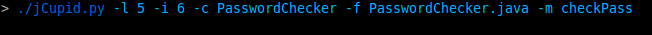
\includegraphics[width=\linewidth]{jCupidCall}
\end{center}

Which tells jCupid that it should use at most 6 random strings of length 5 to run the file PasswordChecker.java
and to examine the method checkPass in the class PasswordChecker. A quick look at that function tells us how
it will check passwords:

\begin{center}
  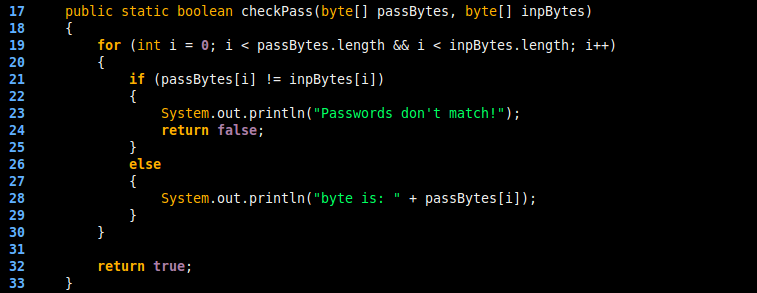
\includegraphics[width=\linewidth]{PasswordChecker}
\end{center}

As we can see this is the simple way of checking passwords, one character at a time and immediately reporting
any failures. This definitely would lead to a timing vulnerability. For reference the password is 
``mySecretPassword'', so we should see some different bytecodes executed between inputs that start with `m'
vs ones that don't. Lets see how jCupid handles this:

\begin{center}
  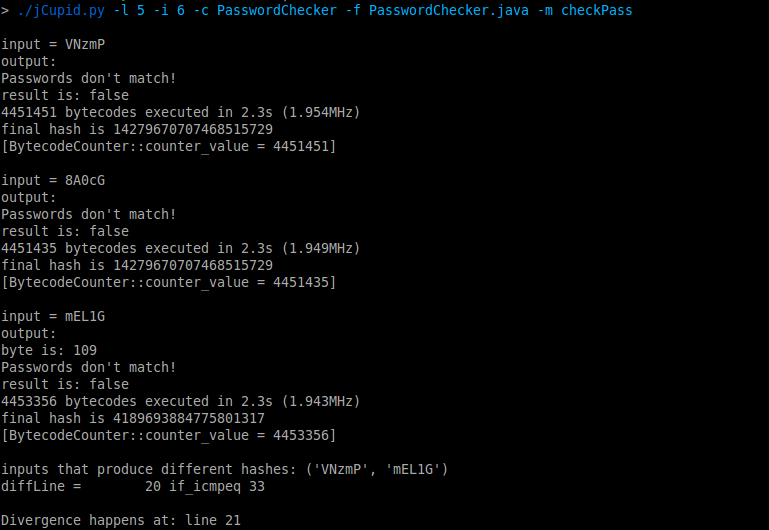
\includegraphics[width=\linewidth]{jCupidRun1}
\end{center}

Here we see that jCupid tells us what it is inputting. The first input is ``VNzmP'', the first character
isn't `m' so we know it will fail immediately. jCupid then shows the output from the program and some
diagnostic output including how many bytecodes were executed and the result of the hash. The second input
is ``8A0cG'' which again should fail immediately and we can see it has the same hash and moves on to the
next input. The third input is ``mEL1G'', this input should lead us down a different path since the first
character matches the first character of our password. Indeed we can see that the hash for this input is
different. This prompts jCupid to now look for the offending bytecode and trace this back to a line in 
the source code, in this case it tells us line 21 is the offending line, which we can see is the line of
the \texttt{if} statement.

The now informed developer can recognize their mistake and fix this code! One common way of ``correctly''
checking passwords is to always loop through the provided password and simply update a counter by and-ing
whether each character matches the correct password. This implementation can be seen here:

\begin{center}
  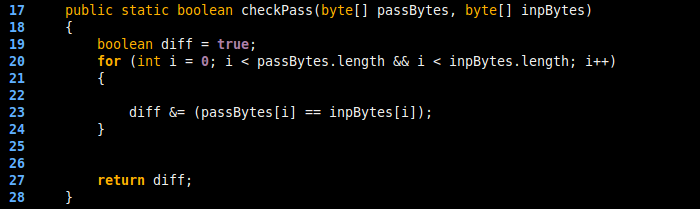
\includegraphics[width=\linewidth]{PasswordCheckerFix1}
\end{center}

This fix looks good! We always examine the full length of the input and are simply updating a variable
with the exact same line of code no matter what. Lets see what jCupid says:

\begin{center}
  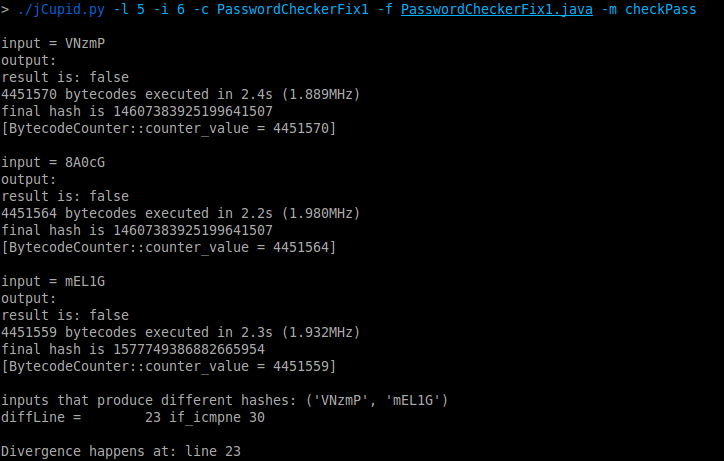
\includegraphics[width=\linewidth]{jCupidRun2}
\end{center}

Running the same inputs through again we see that indeed the two first inputs do the same work, as expected,
but suprisingly we still get different bytecodes executed with this fixed solution. After much investigation
it appears that a peculiarity of Java turns the $==$ into an if statement! Luckily we ran the code through
jCupid again. After some clever thinking we may realize that we need to do this checking without actually
comparing the characters, but we can do a computation on them. Specifically we can xor each character to
determine if they are the same, and then keep a running \texttt{or} to keep track of any differences showing
up. So the code now looks like:

\begin{center}
  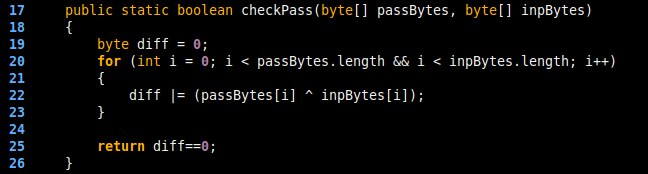
\includegraphics[width=\linewidth]{PasswordCheckerFix2}
\end{center}

Now there are no decisions being made at all in the code, just a computation being done, and the same 
computation. Lets see if jCupid agrees with us:

\begin{center}
  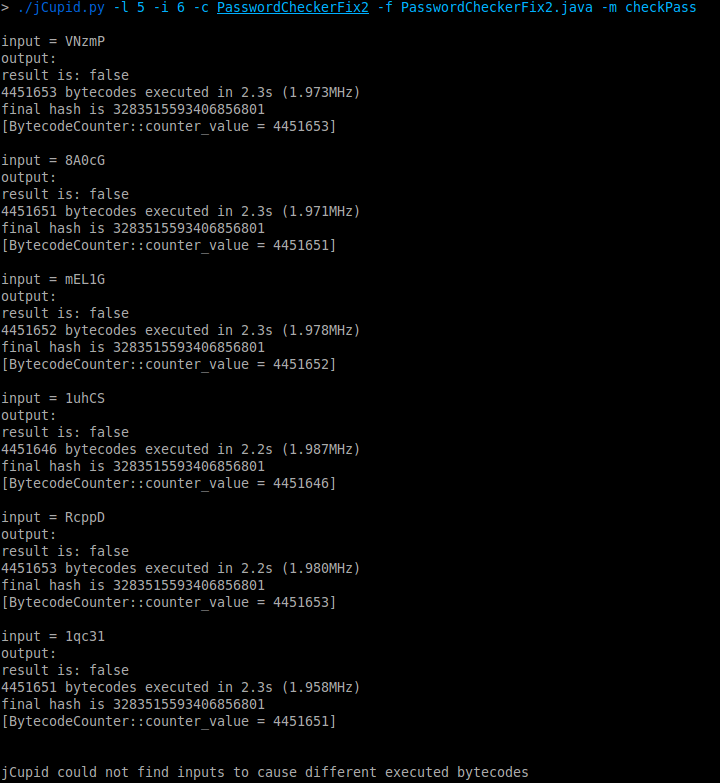
\includegraphics[width=\linewidth]{jCupidRun3}
\end{center}

Indeed we can see that jCupid found no difference between any of the inputs, regardless of whether they 
began the same as the password. Of course we would want to run significantly more trials on numerous 
length inputs in order to be more confident, but we can see that we have fixed our problem of matching
letters causing different instructions to be executed. Even though the first solution we had seemed like
it was exactly what we wanted, Java's compiler changes the code in subtle ways that can add side-channels.

It is worth noting that jCupid can be fooled by using some built-in java libraries. Examine this version
of checking passwords, by simply comparing strings:

\begin{center}
  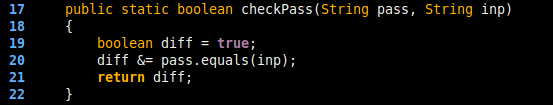
\includegraphics[width=\linewidth]{PasswordCheckerFix3}
\end{center}

Why bother going through the process of comparing strings yourself when Java provides a built-in call for
this? Lets see what jCupid thinks:

\begin{center}
  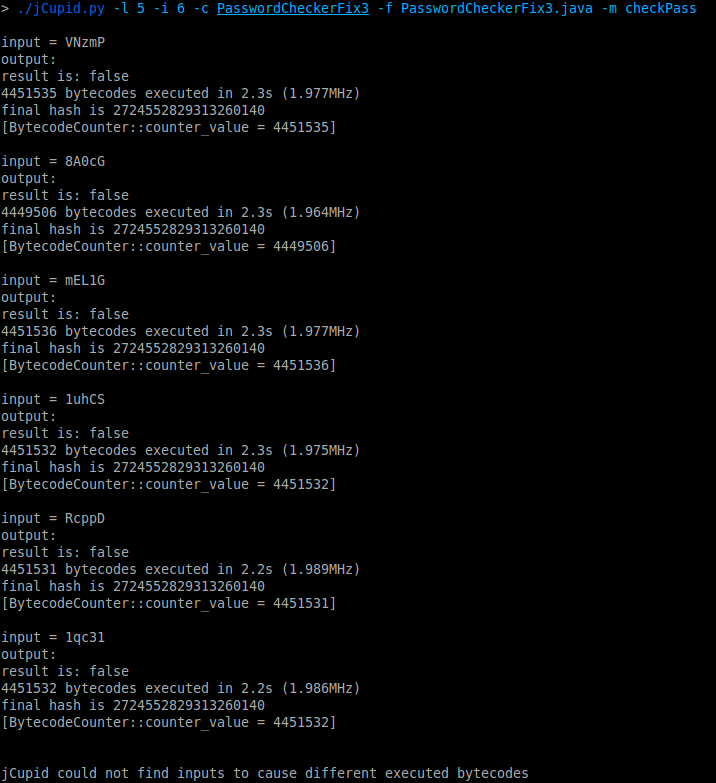
\includegraphics[width=\linewidth]{jCupidRun4}
\end{center}

It appears that all is well! jCupid doesn't notice any difference by using Java's built-in string comparison!
However after some investigation: a significant portion of Java's built-in calls are implemented in \texttt{C++}
meaning that jCupid can't detect any differences, since it only looks at the bytecodes that Java executes. And
in fact Java's built-in methods are not designed to be used in secure applications.

We provide another example: sometimes users code may not have any branches at all, but still input has an effect
on what is computed. In certain situations some inputs can cause more work to be done. In particular consider
the contrived program that reads a string from input and then sums the characters of the string to determine
how many bytes to read from a file and then hash.

Even two inputs of the same size can lead to different bytecodes being executed. So our sample program has
the following structure:

\begin{center}
  \begin{lstlisting}[language=Java]
  public class SumRandomBytes
  {
    public static void main(String [] args)
     {
       Scanner sc = new Scanner(System.in);
       String s = sc.nextLine();
      
       int sumOfBytes = sumString(s);
       byte[] data = new byte[sumOfBytes];
    
       data = readBytes(sumOfBytes);
 
       MessageDigest md = MessageDigest.getInstance(SHA-1);
       md.digest(data);
    }
 }
 \end{lstlisting}
\end{center}

jCupid catches this as:

\begin{center}
  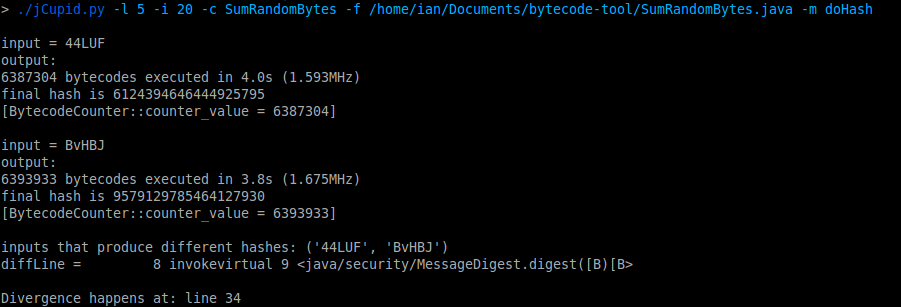
\includegraphics[width=\linewidth]{jCupidSumRandomBytes}
\end{center}

Line 34 corresponds to the \texttt{md.digest(data)} line, which tells us that something is wrong with our
hashing. Of course the issue come from the inputs: \texttt{44LUF} sums to 335 and \texttt{BvHBJ} sums to 
396, thus the first run of our program hashes 335 bytes of data where as the second run hashes 396 bytes,
which leads to a different number of bytecodes executed.
